
現在のアプリ開発は,プログラマのみで完結することは少なく,
多様な背景を持つメンバと協働で行われる.またアプリ開発において,
TrelloやSlackといったICTツールが導入されている.
しかし異なる背景を有するコミュニティのメンバ同士がコミュニケーションを行う場合,
認識論の違いから主張の食い違いや対立が起きることもあるため\cite{conflict},
ICTツールを導入するだけでは異なる背景を持つメンバと協働でアプリ開発を行うには不十分であり,
メンバ間の人間関係がどのように作られていくかといったプロセスも見ていく必要があると考えられる.
そこで実践共同体\cite{Matsumoto}の布置という概念からメンバ間の関係性を捉えることが有効であると考えられる.
布置とは成員は単一の実践共同体のみに参加するものではなく,
複数の実践共同体に参加することを踏まえて,
複数の実践共同体における成員の振る舞いを捉える概念である.
従来の状況論的学習理論における実践共同体\cite{copImg}と布置のイメージを図\ref{cop-overlap}にて示す.

そこで,著者らは実践共同体という概念を用いて,異なる背景を持つプロジェクトメンバが協働でタスクを行うことを支援する手法を提案する.
まず,過去に行った異なる背景を持つプロジェクトメンバの関係構築のあり方が,
開発されるアプリのデザインにどのような影響を及ぼすかという
研究の結果を見直し,課題を明らかにする.
そして明らかになった課題を解決するため,Trello APIからのデータを元にメンバ間の
関係を可視化することにより協働的に作業を促すシステムの提案を行った.

\begin{figure}[h]
  \centering
  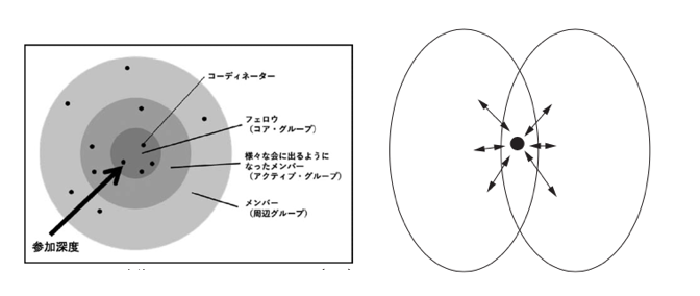
\includegraphics[width=0.5\textwidth]{img/cop-overlap.eps}
  \caption{異なる実践共同体の協働のイメージ図}
  \label{cop-overlap}
\end{figure}
